\begin{figure}[htbp]
\centering
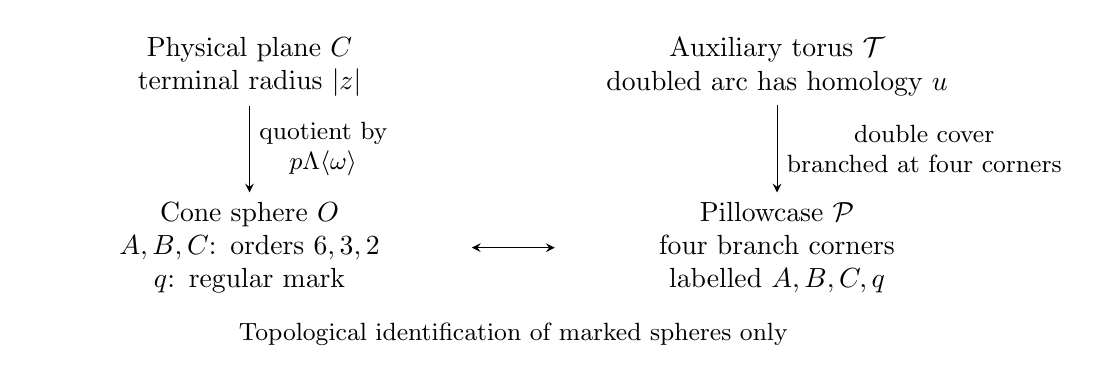
\begin{tikzpicture}[>=stealth, every node/.style={align=center}]
\node[text width=5.4cm] (physical) at (-3.35,2.3)
  {Physical plane \(\mathbb C\)\\terminal radius \(|z|\)};
\node[text width=5.4cm] (cone) at (-3.35,0)
  {Cone sphere \(O\)\\\(A,B,C\): orders \(6,3,2\)\\\(q\): regular mark};
\node[text width=5.4cm] (torus) at (3.35,2.3)
  {Auxiliary torus \(\mathcal T\)\\doubled arc has homology \(u\)};
\node[text width=5.4cm] (pillow) at (3.35,0)
  {Pillowcase \(\mathcal P\)\\four branch corners\\labelled \(A,B,C,q\)};
\draw[->] (physical) -- node[right, font=\small]
  {quotient by\\\(p\Lambda\rtimes\langle\omega\rangle\)} (cone);
\draw[->] (torus) -- node[right, font=\small]
  {double cover\\branched at four corners} (pillow);
\draw[<->] (cone.east) -- (pillow.west);
\node[font=\small] at (0,-1.1)
  {Topological identification of marked spheres only};
\end{tikzpicture}
\caption{The two covering constructions in the radius bound. The auxiliary
torus classifies the endpoint arc by a primitive vector \(u\); its physical
terminal radius is measured in the plane on the left. The identification
of the marked spheres does not identify their metrics or their covers.}
\label{fig:pv:localization-covers}
\end{figure}
